% !TeX spellcheck = de_DE
\documentclass[a4paper, 10pt]{scrartcl}  

\usepackage[width=17.00cm, height=25.00cm]{geometry}
\geometry{verbose,a4paper,tmargin=20mm,bmargin=20mm,lmargin=20mm,rmargin=20mm}

\usepackage[english]{babel}
\usepackage[utf8]{inputenc}
\usepackage{tgcursor}

\usepackage{amsmath,amssymb,amstext}
\usepackage{tikz}
\usepackage{listings}
\usepackage{graphicx}
\usepackage{scrextend}
\usepackage[colorlinks, 				% Inhaltsverzeichnis verlinken
			pdfpagelabels,
			pdfstartview = FitH,
			bookmarksopen = true,
			bookmarksnumbered = true,
			linkcolor = blue!40!black,
			plainpages = false,
			hypertexnames = false,
			citecolor = black] {hyperref}
\usepackage{array}
\usepackage{tcolorbox}
\usepackage{trfsigns}
\usepackage{transparent}
\usepackage{listings}
\usepackage{mcode}

\setcounter{tocdepth}{3}  
\setlength{\arrayrulewidth}{0.1pt}
\setlength{\parindent}{0pt}

% Umrahmung definieren
\tcbset{fonttitle=\bfseries, colback=black!1!,colframe=green!50!black!40!}

\begin{document}
	\begin{titlepage}
		\center 		
		\textsc{\huge \bfseries S-curve Trajektoriengenerator}\\[1cm] 
		\textsc{\Large Generierung und Implementierung einer beschleunigungsbeschränkten Trajektorie für die Sollwertvorgabe}\\[0.5cm] 
		\textsc{\large Author: Bernd Heufelder}\\[0.5cm] 
		{\large \today}\\[1cm] 
		\includegraphics[width=0.3\linewidth]{./pics/BesiLogo.jpg}\\[1cm]
		\begin{flushleft}
			\tableofcontents
		\end{flushleft}
	\end{titlepage}

	\section{Einführung/Motivation}
		Im Gegensatz zu einem Sollwertsprung kann durch Vorgabe einer Solltrajektorie der Verlauf zwischen Anfangssollwert und Endwert beliebig vorgegeben werden. Ziel ist es die Ordnung der überführenden Trajektorie so niedrig als möglich und so groß als nötig zu setzen. 
		
		Zur Sollwertüberführung der Heizertemperatur beim Projekt TGB2 hat sich gezeigt, dass eine lineare Überführung zwischen einer Start- und Endtemperatur für die meisten Anwendung nicht ausreichend ist. Es wird daher im Folgenden die Generierung einer Trajektorie 2. Ordnung behandelt. 
		
		Eine Trajektorie 2. Ordnung wird so verstanden, dass die 2. Ableitung des Sollwertverlaufs konstant ist und der Sollwertverlauf ein Polynom 2. Ordnung darstellt. Wir beschränken also die Beschleunigung des Verlaufs auf einen konstanten Wert $ a_{max} $.
		
		\begin{equation}
			a = [0, \pm a_{max}].
			\label{amax}
		\end{equation}
		
		\begin{figure}[h!]
			\centering
			\includegraphics[width=0.8\linewidth]{./pics/trapez.png}
			\caption{Beschleunigungsbeschränkte Trajektorie mit trapezförmigem Geschwindigkeitsverlauf}
		\end{figure}
		
		Des weiteren sei die 1. Ableitung (Geschwindigkeit) des Verlaufs auf einen vorzugebenden Wert $ v_{lim} $ wie folgt beschränkt
		\begin{equation}
			v = \{v \text{ } | \text{ } -v_{lim} < v < v_{lim}\}.
			\label{vmax}
		\end{equation}
		Mit den Bedingungen \eqref{amax} und \eqref{vmax} ist der zeitlich kontinuierliche Verlauf des Sollwerts durch die Funktion
		\begin{equation}
			T(t) = T_{0} + v\cdot t + \frac{1}{2}a\cdot t^{2}
		\end{equation}
		gegeben. Die Berechnung der S-curve erfolgt durch Integration des Geschwindigkeitsverlaufs. Um diesen Verlauf erstellen zu können, ist die Dauer der Beschleunigungsphasen nötig, welche den gewünschten S-Verlauf ergeben. Als Ansatz für die Erzeugung des Geschwindigkeitsverlaufs, wird zwischen Beschleunigungs-, Konstantgeschwindigkeits- und Verzögerungsphase unterschieden. Bei geringen Überführungsdistanzen kann es abhängig von $ v_{lim} $ und $ a_{max} $ vorkommen, dass $ v_{lim} $ nicht erreicht wird und es somit keine Konstantgeschwindigkeitsphase gibt.
		\begin{figure}[h!]
			\centering
			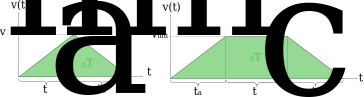
\includegraphics[width=\linewidth]{./pics/bedingungen.png}
			\caption{(links) Grenzfall, bei welchem noch keine Konstantgeschwindigkeitsphase auftritt}
		\end{figure}
		Diese Variation wir anhand einer Fallunterscheidung abgefangen.
	
	\section{Fallunterscheidung}
		Es gibt den Fall, dass die maximale Geschwindigkeit erreicht wird (Fall 1) und es kann vorkommen, dass eine Konstantgeschwindigkeitsphase nicht auftritt (Fall 2).
		
		Falls der zurückgelegte Weg während der Beschleunigungs- und Verzögerungsphase kleiner als die gewünschte Überführungsdistanz ist, dann tritt Fall 1 ein. Wenn diese Bedingung nicht erfüllt ist, dann tritt Fall 2 ein.
		
		\begin{tcolorbox}[title=Bedingung zur Fallunterscheidung]
			Fall 1 tritt ein, sobald die Fläche unter dem Geschwindigkeitsdreieck größer als $ \Delta T $ ist. Mit $ t_{a} \cdot v_{lim}= \Delta T  $ und $ t_{a} = \frac{v_{lim}}{a_{max}} $ als die Zeit bis zum Erreichen des Geschwindigkeitslimits, ergibt sich der Grenzfall, bei welchem noch keine Konstantgeschwindigkeitsphase auftritt. Es ergbit sich folgende Bedingung für Fall 1:\\
			\begin{equation}
				\Delta T > \frac{v_{lim}^{2}}{a_{max}}
			\end{equation}
			mit
			\[ \Delta T = T_{1} - T_{0} \]
			\tcblower
			$ T_{0} $ ... Starttemperatur
			
			$ T_{1} $ ... Zieltemperatur
			
		\end{tcolorbox}		
	
		\subsection{Fall 1}
			Für den Fall mit konstanter Geschwindigkeitsphase setzen wir die benötigte Gesamtüberführungszeit aus drei Teilen zusammen. Dabei wird die Verzögerung gleich der Beschleunigung und somit $ t_{a}=t_{d} $ gesetzt.
			
			\[t_{end} = 2\cdot t_{a} + t_{c}\]
				
			Die Zeit bis zum Erreichen der Konstantgeschwindigkeit ist durch
			\begin{equation}
				t_{a} = \frac{v_{lim}}{a_{max}}
				\label{ta_case1}
			\end{equation}
			gegeben. Die Dauer der Phase mit konstanter Geschwindigkeit kann aus dem Ansatz $ \Delta T = \frac{1}{2}v_{lim}\cdot t_{a} + v_{lim}\cdot t_{c} + \frac{1}{2}v_{lim}\cdot t_{a} $ hergeleitet werden:
			\begin{equation}
				t_{c} = \frac{\Delta T}{v_{lim}} - \frac{v_{lim}}{a_{max}}.
				\label{tc_case1}
			\end{equation}
			 
			
		\subsection{Fall 2}
			Im Fall wo keine Konstantgeschwindigkeit erreicht wird, berechnet sich die erreichte Maximalgeschwindigkeit zu
			\begin{equation}
				v_{a} = a_{max}\cdot t_{a}.
				\label{vmax_case2}
			\end{equation}
			Die Temperaturdifferenz ergibt sich mit
			\[\Delta T = v_{a}\cdot t_{a}\]
			und durch einsetzen von \eqref{vmax_case2} erhält man
			\[\Delta T = a_{max}\cdot t_{a}^{2}.\]
			Daraus kann die benötigte Überführungszeit berechnet werden:
			\[t_{a} = \sqrt{\frac{\Delta T}{a_{max}}} \]
			
	\section{Generierung des diskreten Geschwindigkeitsverlaufs}	
		Mit der Abtastzeit $ t_{s} $ und den Zeiten der einzelnen Phasen, $ t_{a} $ für Fall 2 und $ t_{a},t_{c} $ für Fall 1, kann die Anzahl der Punkte pro Phase berechnet werden.\\\\
		
		\begin{minipage}{0.45\textwidth}
			Fall 1:
			\[n_{a} = round\bigg(\frac{t_{a}}{t_{s}}\bigg)\]
			\[n_{c} = round\bigg(\frac{t_{c}}{t_{s}}\bigg)\]
			\[n = 2\cdot n_{a} + n_{c}\]
		\end{minipage}%
		\hfill
		\begin{minipage}{0.45\textwidth}
			Fall 2:
			\[n_{a} = round\bigg(\frac{t_{a}}{t_{s}}\bigg)\]
			\[n = 2\cdot n_{a}\]
		\end{minipage}\\\\
	
		Durch die Diskretisierung des Verlaufs ergibt sich zwangsweise eine Abweichung zum kontinuierlichen Verlauf. Dieser Fehler soll durch Anpassung von $ v_{lim}$ und $a_{max} $ minimiert werden. Durch die Ganzzahlige Anzahl an Punkten pro Phase, ergeben sich minimal unterschiedliche Dauern der Phasen. Diese gerundeten Phasenzeiten werden im Folgenden durch eine Tilde $ \tilde{t} $ gekennzeichnet. \\\\
		
		\begin{minipage}{0.45\textwidth}
			Fall 1:
			\[\tilde{t}_{a} = n_{a}t_{s}\]
			\[\tilde{t}_{c} = n_{c}t_{s}\]
			\[\tilde{t}_{end} = (n_{a}+n_{c})t_{s}\]
		\end{minipage}%
		\hfill
		\begin{minipage}{0.45\textwidth}
			Fall 2:
			\[\tilde{t}_{a} = n_{a}t_{s}\]
			\[\tilde{t}_{end} = 2\cdot n_{a}t_{s}\]
		\end{minipage}\\\\
	
		Um eine exakte Überführungsdistanz $ \Delta T $ zu garantieren, können nun die Parameter $ v_{lim} $ und $ a_{max} $ so angepasst werden, dass sich mit den neuen Werten $ \tilde{t}_{a},\tilde{t}_{c},\tilde{v}_{lim}, \tilde{a}_{max} $ wieder exakt das vorgegebene $ \Delta T $ ergibt.\\\\ 
		
		\begin{minipage}{0.45\textwidth}
			Fall 1:
			\[\tilde{a}_{max} = \dfrac{\Delta T}{\tilde{t}_{a}(\tilde{t}_{a}+\tilde{t}_{c})}\]
			\[\tilde{v}_{lim} = \tilde{a}_{max}\tilde{t}_{a}\]
		\end{minipage}%
		\hfill
		\begin{minipage}{0.45\textwidth}
			Fall 2:
			\[\tilde{a}_{max} = \dfrac{\Delta T}{\tilde{t}_{a}^{2}}\]
			\[\tilde{v}_{lim} = \tilde{a}_{max}\tilde{t}_{a}\]
		\end{minipage}\\\\
		
		\begin{figure}[h!]
			\centering
			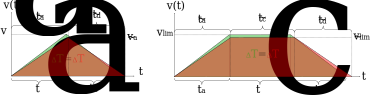
\includegraphics[width=\linewidth]{./pics/bedingungen_tilde.png}
			\caption{Visualisierung der Anpassung von $ v_{lim} $ und $ a_{max} $ auf $ \tilde{v}_{lim} $ und $ \tilde{a}_{max} $}
		\end{figure}
		Mit diesen angepassten Parametern $ \tilde{v}_{lim} $ und $ \tilde{a}_{max} $ kann nun der Geschwindigkeitsverlauf vorgegeben werden, mit welchem dann möglichst gut $ T_{1} = T_{0} + \Delta T $ gilt. In Matlab oder Python kann dieser Geschwindigkeitsverlauf beispielsweise mit Hilfe der Funktion \textit{linspace} bzw. \textit{numpy.linspace} erzeugt werden. Durch einfache Integration, z.b. mittels der Trapezregel, erhält man dann die gewünschte S-curve zwischen $ T_{0} $ und $ T_{1} $.
		\[ T(k) = T(k-1) + t_{s}\dfrac{v(k) + v(k-1)}{2}    \]
		mit 
		\[ T(0) = T_{0}.\]
		
	
	\section{Abschätzung des maximalen Fehlers zu $ v_{lim} $ und $ a_{max} $ (work in progress)}
	
		\subsection{Fall 1}
			\[\Delta a_{max} = \Delta T \bigg(\frac{1}{t_{a}(t_{a}+t_{c})} -  \frac{1}{\tilde{t}_{a}(\tilde{t}_{a}+\tilde{t}_{c})}\bigg)\]
			\begin{figure}[h!]
				\centering
				\includegraphics[width=0.9\linewidth]{./pics/err_acc.png}
				\caption{Abweichung der angepassten Beschleunigung $ \tilde{a}_{max} $ zur Vorgegebenen $ a_{max} $ in Abhängigkeit der Beschleunigungs- und Konstantgeschwindigkeitszeit $ t_{a}, t_{c} $ und $ \Delta T $}
			\end{figure}
			Es ist ersichtlich, dass die Abweichung erst relevant wird, wenn $ t_{a},t_{c} $ klein im Vergleich zum maximalen Rundungsfehler $ \Delta t_{a,max}=\Delta t_{c,max}=0.4\dot{9}t_{s} $ werden. Dieser Fall tritt auf, wenn entweder die Beschleunigung $ a_{max} $ und die Geschwindigkeitsbeschränkung $ v_{lim} $ groß werden oder $ \Delta T $ sehr klein. 
			
		\subsection{Fall 2}
			 \[\Delta a_{max} = \Delta T \bigg(\frac{1}{t_{a}^{2}} -  \frac{1}{\tilde{t}_{a}^{2}}\bigg)\]
			\begin{figure}[h!]
				\centering
				\includegraphics[width=0.9\linewidth]{./pics/err_acc_case2.png}
				\caption{Abweichung der angepassten Beschleunigung $ \tilde{a}_{max} $ zur Vorgegebenen $ a_{max} $ in Abhängigkeit der Beschleunigungszeit von $ t_{a} $ und $ \Delta T $}
			\end{figure}
			Für den Fall 2 gilt: Eine große Abweichung der angepassten Beschleunigung zur Vorgegebenen tritt auf, wenn das $ \Delta T $ groß und $ t_{a} $ klein, also $ a_{max} $ groß, wird. Da keine großen Beschleunigungen vorkommen, ist auch dieser Fall zu vernachlässigen.
			\pagebreak
		
	\section{Code Implementierung}
		\subsection{Matlab}
			
			\lstinputlisting{scurve.m}
			
\end{document}